\documentclass[a4paper,twoside,11pt]{article}
\usepackage[utf8]{inputenc}
\usepackage{graphicx}
\usepackage{url}
\usepackage{epsfig}
\usepackage{natbib}

% pdflatex

% redefinição das margens das páginas
\setlength{\textheight}{24.00cm}
\setlength{\textwidth}{15.50cm}
\setlength{\topmargin}{0.35cm}
\setlength{\headheight}{0cm}
\setlength{\headsep}{0cm}
\setlength{\oddsidemargin}{0.25cm}
\setlength{\evensidemargin}{0.25cm}

\title{D\'{A}DIVA IPO\\\large Digital Aid and Donor Information Verification Application for IPO}

\author{
\begin{tabular}{c}
             Francisco Medeiros, n.º 46631, e-mail: a46631@alunos.isel.pt, tel.: 913192828\\
             Luís Macário, n.º 47671, e-mail: a47671@alunos.isel.pt, tel.: 933694131\\
			 Ricardo Pinto, n.º 47673, e-mail: a47673@alunos.isel.pt, tel.: 927111044\\
\end{tabular}}

\date{
\begin{tabular}{ll}
  {Supervisors:} & Filipe Freitas, e-mail: filipe.freitas@isel.pt \\
                 & João Pereira, e-mail: joaomiguel.pereira@cofidis.pt, Cofidis\\
\end{tabular}\\
\vspace{5mm}
\today}

\begin{document}

\maketitle

\section{Introduction}
Today, the professionals at the Instituto Português de Oncologia (IPO) in Lisbon, within the blood donor service, rely on paper to consult some of the information needed to screen donors. The aim is to create a search portal to properly classify and index information, which will return contextualized results ordered by relevance. This part of the portal will be collaborative, allowing for peer-reviewed information. The portal could also allow the donors to quickly register in the donor system and fill out the pre-donation form. The objective would be to significantly decrease the possibilities of mistakes that storing information in a paper format brings, as well as decrease the time it takes to donate blood by fast-tracking the signup and triage processes.

\section{System Requirements}
\subsection{Functional Requirements}
\begin{description}
	\item[Authentication and Authorization]- The Portal may have an anonymous area aimed at consultation or the presentation of institutional information, but the main areas will require user authentication and the functionalities will be made available through user permissions.
	\item[Back Office]- The portal will have a back office used for configuring portal parameters. User management will be one of the features of this back office.
	\item[Workflow for classifying and submitting information with peer review]- Changes made by a user must be approved by another user to guarantee their relevance and accuracy before being integrated into the search results.
	\item[Google-like search and results by relevance]- Search should be as simple as possible. There may be a need to increase the number of filters, but this complexity should be hidden. The results returned should be sorted based on relevance.
	\item[Donation registration form]- Donors should be able to quickly fill out a digital sign-up form that automatically inputs their data into the system.
\end{description}

\subsection{Non-Functional Requirements}
\begin{enumerate}
	\item Intuitive user experience through a simple user interface and practical/password-less authentication methods.
	\item The platform will have a digital questionnaire with a few questions about previous illnesses, medication use, recent trips, and other factors that could compromise a safe donation.
	\item Clear documentation and as automated as possible to ensure it's always up to date.
	\item Software testing to increase our confidence in the system’s security and features. It should also allow us to move faster without fear of breaking the previous working code.
	\item Overall good software practices that should allow the system to grow in complexity more easily.
	\item Service scalability. Making it possible to spin up the new servers running our service in parallel to increase overall system performance and availability.
	\item Deploying the application components and making them available to the public.
\end{enumerate}

\subsection{Optional Features}
\begin{enumerate}
	\item On donation scheduling, automatically check vaccination and medication prescription over the last 6 months and cross-check the results with known compounds that warrant a blood donation waiting period, as well as adding tags to donations with the donor's current medication, if any, to check for possible donation recipient allergies or other complications. Would require integration with an external service (Most likely SNS) to receive the donor’s medical history.
	\item Users can authenticate using the Digital Mobile Key (CMD). Would require integration with the AMA (Administrative Modernization Agency) systems.
\end{enumerate}

\section{Technologies}
We plan to use ASP.NET to build the Web API, following DDD (Domain Driven Design) and using the Minimal API architecture. We will use NodeJS and React.js to deliver the front-end experience. We will use ElasticSearch to store the donor’s data and the contextualized information. ElasticSearch will be used due to its searching capabilities, returning search results based on a relevance algorithm.

\section{Risks}
Some factors that might influence our speed on the project development are:
\begin{enumerate}
	\item C\# and .NET are technologies that we’re not experienced in, resulting in some time being needed for adaptation.
\end{enumerate}

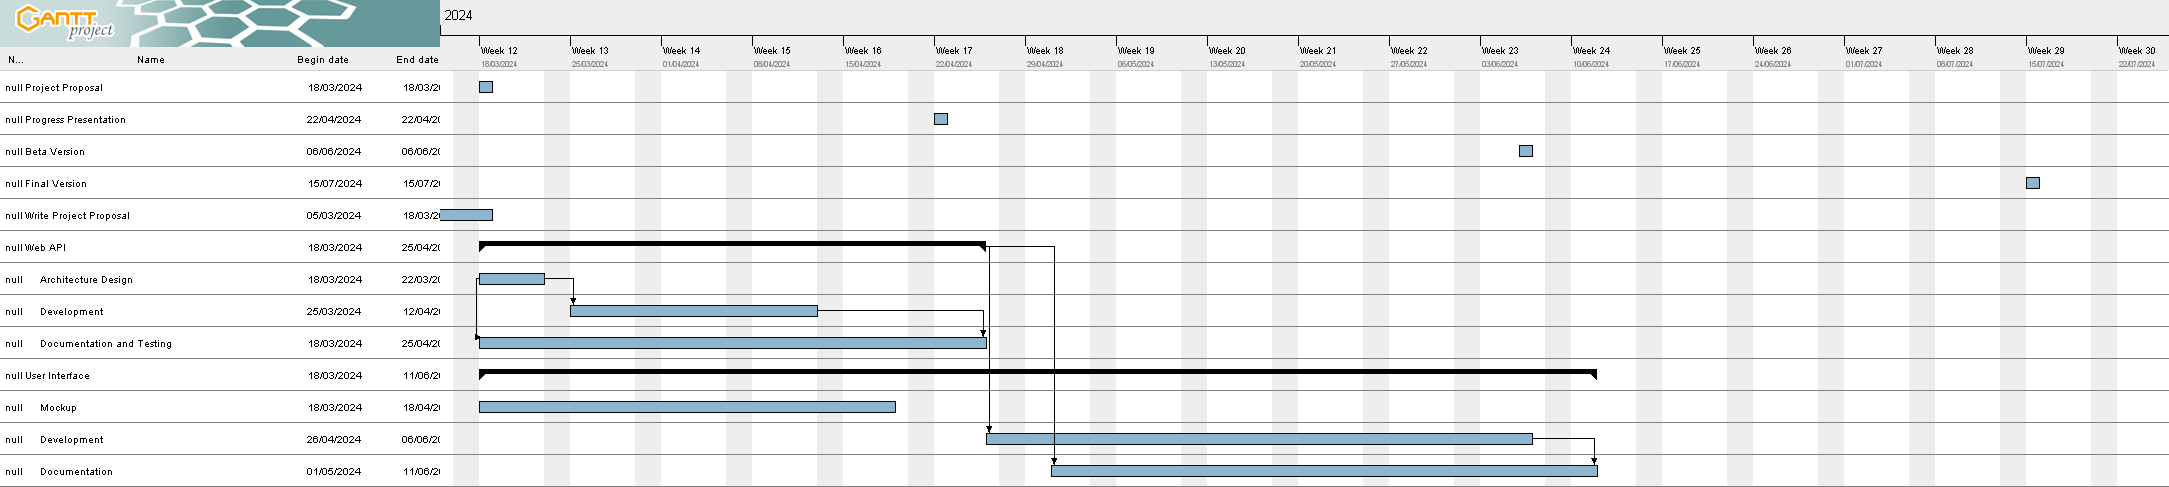
\includegraphics[width=15cm]{gantt.png}

\bibliographystyle{unsrt}
\bibliography{references}

\end{document}